\label{Wireshark Handling}
\chapter{Wireshark Handling}
Explain what we are going to do in this section here

\section{Provide a short documentation that explained its actions}

Wireshark is a network protocol analayzer. Using wireshark, we can monitor what's happeing on the network.
\paragraph{}
\textbf{Who use Wireshark?}
\begin{itemize}
\item Network administrators use it to troubleshoot network problems
\end{itemize}
\begin{itemize}
\item Network security engineers use it to examine security problems
\item QA engineers use it to verify network applications
\item Developers use it to debug protocol implementations
\item People use it to learn network protocol internals 
\end{itemize}

\textbf{Featues}

\begin{itemize}
\item Available for UNIX and Windows.
\item it is an open source software project, and is released under the GNU General Public License (GPL)
\item Capture live packet data from a network interface including Ethernet, Wireless LAN,…
\item Open files containing packet data captured with tcpdump/WinDump, Wireshark, and many other packet capture programs.
\item Import packets from text files containing hex dumps of packet data.
\item Display packets with very detailed protocol information.
\item Save packet data captured.
\item Export some or all packets in a number of capture file formats.
\item Filter packets on many criteria.
\item Search for packets on many criteria.
\item Colorize packet display based on filters.
\item Create various statistics.
\end{itemize}
\textbf{Wireshark is not}
\begin{itemize}
\item It  isn’t an intrusion detection system. It will not warn you when someone does strange things on your network . However, if it happens, Wireshark can help you figure out what is really going on.
\item Wireshark will not manipulate things on the network..  Wireshark doesn’t send packets on the network.
\end{itemize}

\textbf{Supported platforms}

Wireshark runs on most UNIX and UNIX-like platforms including Linux and most BSD variants. It also runs on various Windows platforms.

\clearpage
\section{ How long was the period between the sending of the HTTP GET message until the
receipt of the HTTP OK reply? Provide screenshots}


\begin{figure}[H]
\centering
  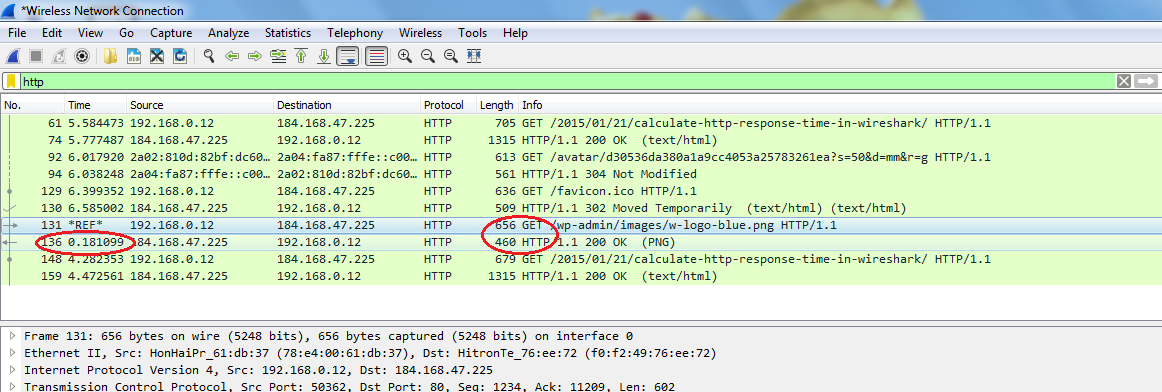
\includegraphics[width=.9\textwidth]{Images/Task1_1.png}
  \caption{Http Response Time is 183 ms.}
  \label{fig:1.1}
\end{figure}

\section{What are the IP addresses of the servers www.fau.de and www.denic.de?}

www.fau.de: 131.188.16.209 , 
www.denic.de: 81.91.170.12

\begin{figure}[H]
\centering
  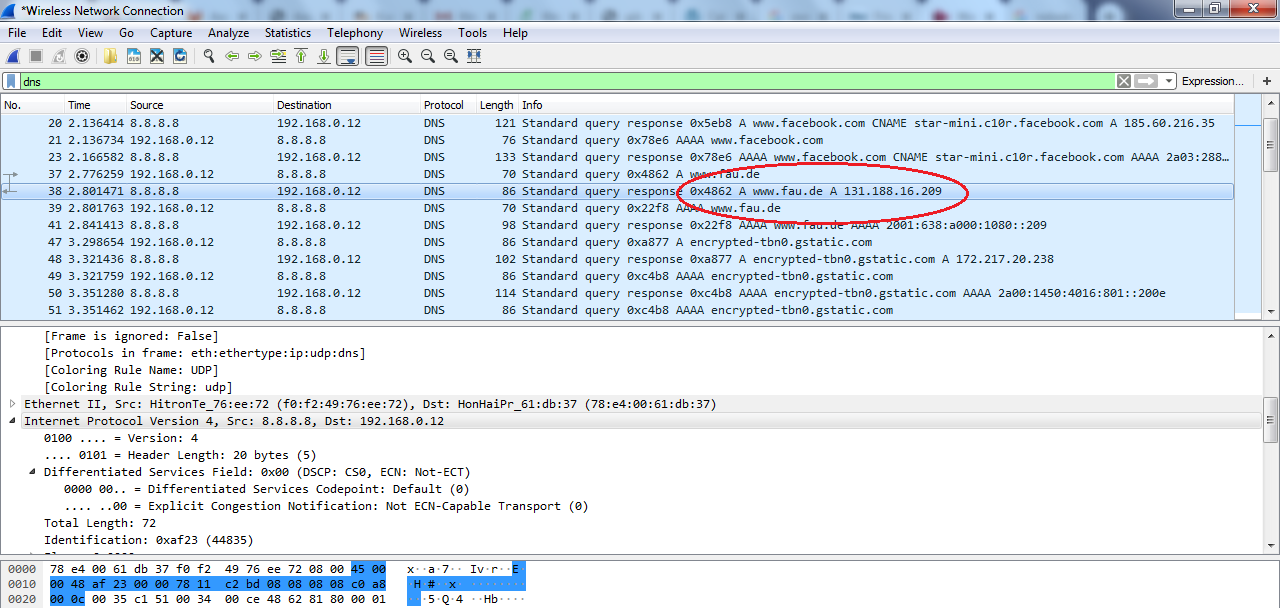
\includegraphics[width=.9\textwidth]{Images/Task1_2_fau.de.png}
  \caption{fau.de IP Address}
  \label{fig:1.2}
\end{figure}



\begin{figure}[H]
\centering
  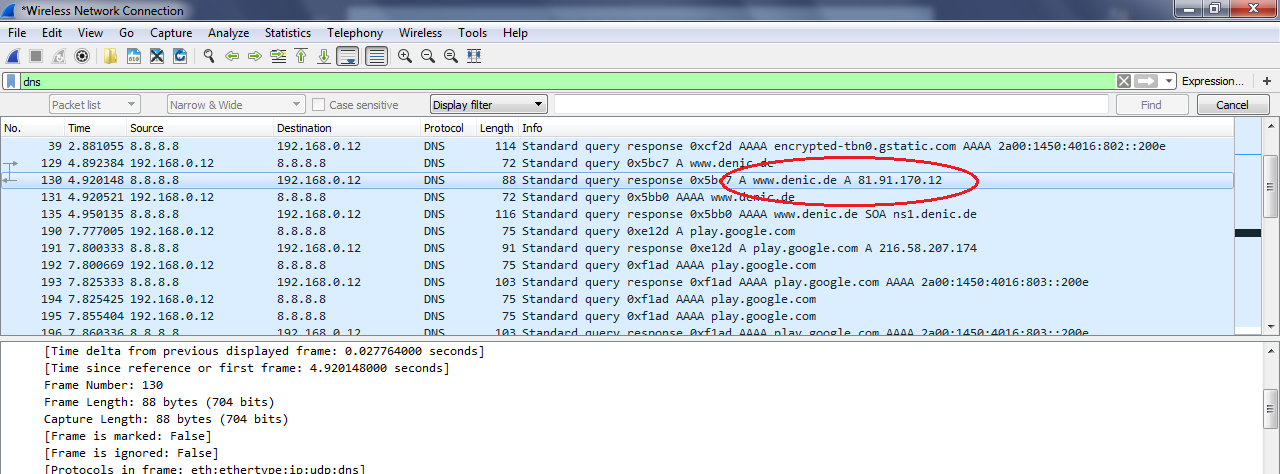
\includegraphics[width=.9\textwidth]{Images/Task1_2_denic.de.png}
  \caption{denic.de IP Address}
  \label{fig:1.3}
\end{figure}

%  if you want to make new paragaph u can simply write \paragraph{} and then what u want to write